\section{Differential expression and pathway-level follow-up}
We re-ran the airway dexamethasone experiment (GEO GSE52778) through the sugarcode DESeq2 path and through PyDESeq2. Of 16,802 genes passing the count filter, the paired design $\sim$cell$+$dex gave 4,451 genes at adjusted $p<0.05$ and the unpaired design gave 3,203. Size factors agreed to a maximum relative difference of 1.8e-09 (benchmarks/sweep\_de\_pydeseq2.json).
\paragraph{(F25) Negative-binomial GLM.} For gene $g$ and sample $j$, $K_{gj}\sim\mathrm{NB}(\mu_{gj},\alpha_g)$ with $\mu_{gj}=s_j q_{gj}$ and $\log_2 q_{gj}=\sum_r x_{jr}\beta_{gr}$, so $\mathrm{Var}(K_{gj})=\mu_{gj}+\alpha_g\mu_{gj}^2$.
\paragraph{(F26) Median-of-ratios size factor.} $s_j=\mathrm{median}_{g:K_{g\cdot}>0}\, K_{gj}\big/\big(\prod_{v=1}^{m}K_{gv}\big)^{1/m}$.
\paragraph{(F27) Wald statistic.} $W_g=\hat\beta_{g,\mathrm{dex}}/\mathrm{SE}(\hat\beta_{g,\mathrm{dex}})$, compared with $N(0,1)$; the paired design removes the cell-line effect from the residual variance, which is why it finds more genes than the unpaired design.
\subsection{Gene-set over-representation}
We took the 536 dex-induced genes (adjusted $p<0.05$, $\log_2\mathrm{FC}>1$) and tested them against the 16,802 tested genes with g:Profiler (version e114\_eg62\_p19\_27110d83, g:SCS correction). 31 terms passed. The top terms are broad (Table~\ref{tab:gost}).
\paragraph{(F28) Hypergeometric tail.} With background size $M$, term size $K$, query size $n$ and overlap $k$, $p=\sum_{i\ge k}\binom{K}{i}\binom{M-K}{n-i}\big/\binom{M}{n}$, and fold enrichment $=(k/n)/(K/M)$.
\begin{table}[h]\centering\small\begin{tabular}{llrrr}\hline Source & Term & overlap & size & $p_{\mathrm{adj}}$\\\hline
GO:BP & multicellular organismal process & 228 & 4764 & 2.8e-07\\
GO:BP & signaling & 209 & 4354 & 4e-06\\
GO:BP & cell communication & 209 & 4365 & 5.2e-06\\
GO:BP & cell adhesion & 73 & 1031 & 1.5e-05\\
GO:BP & system process & 80 & 1189 & 2.1e-05\\
GO:BP & response to stimulus & 261 & 5987 & 8.6e-05\\
GO:BP & signal transduction & 192 & 4028 & 8.9e-05\\
GO:BP & anatomical structure development & 196 & 4191 & 0.00027\\
GO:BP & cell migration & 74 & 1134 & 0.00041\\
KEGG & Cytoskeleton in muscle cells & 19 & 172 & 0.00042\\
GO:BP & developmental process & 209 & 4580 & 0.00047\\
GO:BP & cell differentiation & 152 & 3041 & 0.00054\\
\hline\end{tabular}\caption{Top g:Profiler terms for dex-induced genes (benchmarks/sweep\_dex\_enrichment.json).}\label{tab:gost}\end{table}
\paragraph{Negative result.} The terms one would expect for a glucocorticoid are enriched but do not survive correction:
\begin{table}[h]\centering\small\begin{tabular}{lrrrr}\hline Term & overlap & size & fold (approx.) & $p_{g:SCS}$\\\hline
cellular response to glucocorticoid stimulus & 9 & 43 & 7.16 & 0.43\\
response to corticosteroid & 10 & 91 & 3.76 & 1\\
response to glucocorticoid & 10 & 81 & 4.22 & 1\\
cellular response to corticosteroid stimulus & 9 & 48 & 6.42 & 1\\
\hline\end{tabular}\caption{Glucocorticoid terms: large fold change, not significant. }\end{table}
The small term sizes (tens of genes) and the strong multiple-testing burden explain this: a 7-fold enrichment built on 9 genes is not enough evidence after g:SCS correction. We report it as a negative rather than as confirmation of the expected biology.
\subsection{Reactome pathways}
Reactome AnalysisService mapped the query to 1,098 pathways (240 identifiers not found). No pathway reached FDR$<0.05$; the smallest FDR was 0.11. Reactome uses its whole human gene universe as background, which is a further caveat.
\begin{table}[h]\centering\small\begin{tabular}{lrrrr}\hline Pathway & found & total & $p$ & FDR\\\hline
Anchoring fibril formation & 5 & 15 & 0.00037 & 0.11\\
FOXO-mediated transcription & 13 & 110 & 0.00056 & 0.11\\
Laminin interactions & 7 & 31 & 0.00028 & 0.11\\
Metallothioneins bind metals & 5 & 16 & 0.00049 & 0.11\\
Non-integrin membrane-ECM interactions & 12 & 83 & 0.00015 & 0.11\\
Collagen chain trimerization & 8 & 44 & 0.00044 & 0.11\\
FOXO-mediated transcription of oxidative stress, m & 8 & 49 & 0.00087 & 0.13\\
Adipogenesis & 15 & 147 & 0.00096 & 0.13\\
Degradation of the extracellular matrix & 15 & 148 & 0.001 & 0.13\\
Response to metal ions & 5 & 21 & 0.0016 & 0.17\\
\hline\end{tabular}\caption{Top Reactome pathways (benchmarks/sweep\_dex\_reactome.json).}\end{table}
\paragraph{(F29) Benjamini-Hochberg.} For ordered $p_{(1)}\le\dots\le p_{(m)}$, $q_{(i)}=\min_{j\ge i}\min\{1,\,m\,p_{(j)}/j\}$.
\subsection{Protein interaction network}
STRING's PPI enrichment test on the top 300 dex-induced genes mapped 284 proteins with 402 edges against 184 expected (average degree 2.83, local clustering 0.368), reported $p$ below floating-point resolution. Caveat: STRING's expectation uses a genome-wide background, so genes expressed in airway smooth muscle may be more connected than random genes regardless of dex.
\paragraph{(F30) Edge enrichment ratio.} $E=\,$observed edges$/$expected edges$=402/184=2.18$.
\section{Pairwise alignment against parasail}
We aligned all 300 pairs of 25 protein sequences with sugarcode and parasail 2.6.1. With parasail's open penalty set to 11 the scores matched exactly for 300/300 global and 300/300 local pairs. With open penalty 12 only 36 and 65 matched (maximum difference 26 and 5). This fixes the convention: sugarcode's gap\_open$=-11$ is the cost of the first gap residue, i.e. parasail open 11.
\paragraph{(F31) Affine gap cost.} A gap of length $L$ costs $\gamma(L)=o+(L-1)e$ under sugarcode and parasail open$=11$; under the alternative convention $\gamma(L)=o+Le$, which explains the open-12 mismatch.
\begin{figure}[h]\centering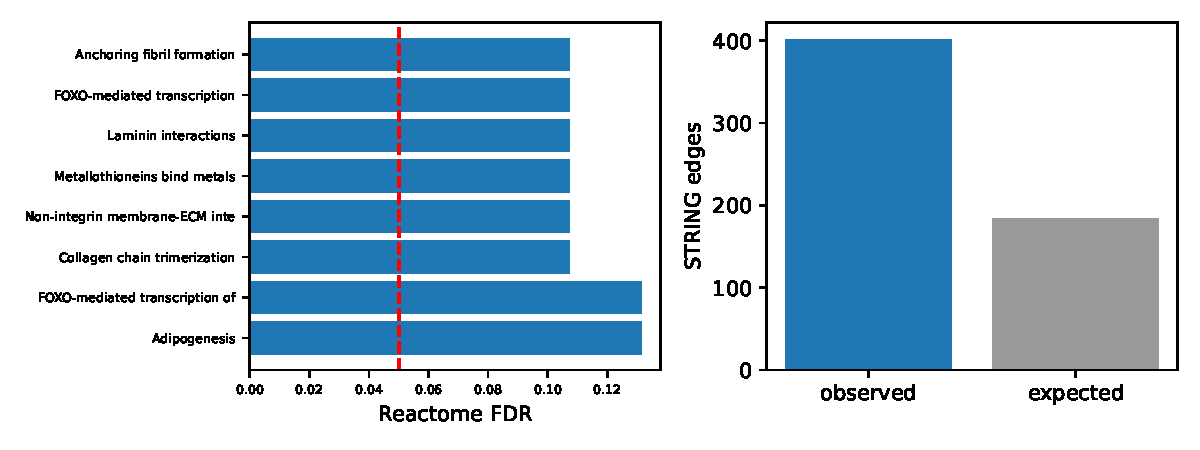
\includegraphics[width=0.95\textwidth]{figs/dex_pathways.pdf}\caption{Left: Reactome FDRs for the top pathways; the red line is 0.05. Right: STRING observed versus expected edges.}\end{figure}
